\subsection{Kubernetes for NFV}
	
\begin{flushleft}
    Kubernetes is a production-grade, open-source infrastructure for the deployment, scaling, management, and composition of application containers across clusters of hosts \cite{k8sarch}. Kubernetes provides facilities to deploy and manage applications that utilize multiple containers. As highlighted in \cite{k8sarch}, the key design goals for kubernetes include portability, generality, legacy support, flexibility, extensibility, and automation possibility. 
\end{flushleft}

\begin{figure}
    \centering
    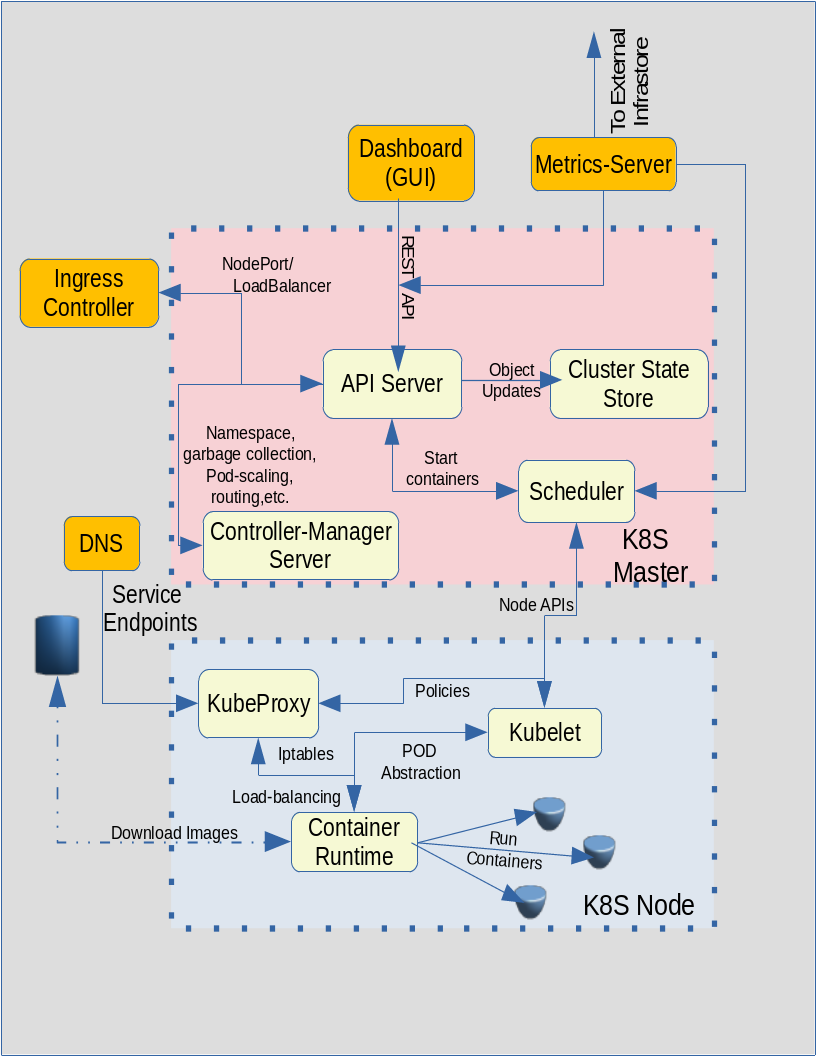
\includegraphics[width=0.5\textwidth]{kubernetes_arch}
    \label{fig:figure16}
    \caption{A block diagram representation of Kubernetes components. Derived from the description in \cite{k8sarch}}
\end{figure}

The architecture involves two types of nodes:
\begin{itemize}
    \item Kubernetes Master also known as the Cluster Control Plane
    \item Kubernetes Node that runs the containers and worloads
\end{itemize}

The Kubernetes Master provides interface to the user and maintains the state of the cluster. The control system of the master and the slave nodes work on the level-based principle wherein they act on drivin the state of the system to a desired state. They react to changes in the state through events and avoid redundant operations and minimizing reaction latency \cite{k8sarch}.
The Master node components can either be all run in a single machine or can be distributed to achieve high availability and load balancing capabilities.
The fundamental unit of kubernetes deployment is called a "POD" which is a group of containers running on the Kubernetes nodes.


The Master node comprises of the following components:

\begin{enumerate}
    \item \textit{API Server}
        It exposes the administrative functions of the Kubernetes cluster through REST API. 
    \item \textit{Cluster State Store}
        A service like etcd that stores all cluster related information persistently in a key-value format.
    \item \textit{Controller-Manager Server}
        Most of the cluster functions like creation, lifecycle management, garbage collection and the API business logic are implemented by Controller Managers. The Controller Manager is a daemon that watches the kubernetes state and makes changes to achieve the desired state. Kubernetes ships with controllers like \textit{replication controller, endpoints controller, namespace controller} and \textit}{serviceaccounts controller} \cite{k8scntmng}.
    \item \textit{Scheduler}
        The Kubernetes scheduler is responsible to choose from a set of hosts to start a set of containers for an application on request. The user can specify constraints on resource availability, Quality of Service, affinity and anti-affinity which are taken into account by the scheduler for allocation. The Scheduler also watches unscheduled PODs and binds them to nodes \cite{k8sarch}. 
\end{enumerate}

The Kubernetes node components provide the required services to run applications on containers or a group of containers(PODs). It includes the following 3 main components:

\begin{enumerate}
    \item \textit{Kubelet}
        Kubelet implements the PODs and Node APIs. PODs can host multiple containers with shared storage volumes and network infrastructure. The POD contains all the necessary resources for the application to run. All containers in a POD share a single IP address and port space and a "localhost" address is used to communicate with each other. The PODs are identified by a unique ID UUID and bind to a node until terminated. In case of faults, a new identical POD is created and the earlier POD is not rescheduled \cite{k8spod}. Through the Node APIs, Kubelet provides the essential mechanism for admission control. 
    \item \textit{Container runtime}
        Every node has a container runtime responsible for getting the images and running the containers \cite{k8sarch}. The container runtime is a logical equivalent of a hypervisor in virtualization. A CRI (Container Runtime Interface) integrates with Kubelet with the help of specifications, protobuf API and libraries that provide service management, request management and caching and error management services \cite{k8scri}. Kubernetes currently supports following CRIs:
        \begin{itemize}
            \item Docker
            \item CRI-O
            \item frakti
            \item rktlet
            \item cri-containerd
        \end{itemize}
    \item \textit{Kube Proxy}
        The kube proxy provides a mechanism to group PODs and apply iptables policies and load balancing. The services are discovered through interaction with the DNS service.
\end{enumerate}

In addition to the above components, a Kubernetes system can also use additional components to help its operations:
\begin{enumerate}
    \item \textit{DNS} - Provides name service for service PODs
    \item \textit{Ingress Controller} - Proivdes access to services by external entities
    \item \textit{Metrics-Sever} - Provides collection and monitoring of metric data on running PODs
    \item \textit{Dashboard} - Provides a Graphical User Interface for the administrative tasks on the Kubernetes cluster.
\end{enumerate}

Kubernetes is a relatively new introduction to the NFV world. The network functions that are made to run in a container are referred to as Containerized Network Functions (CNFs). The CNCF (Cloud Native Computing Federation) is constantly striving to enable Kubernetes as an alternative technology to realize NFV Infrastructure. [\cite{sharma16}] provides a comprehensive comparison of Containers vs Virtual Machines and establishes that containers are a viable option for realizing NFV use-cases.
